\section{The Rectification}

\begin{wrapfigure}{rt}{.3\textwidth}
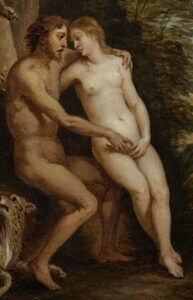
\includegraphics[width=.3\textwidth]{AdamAndEveInParadiseTN-1-193x300.jpg}
\end{wrapfigure}

In the Introduction to \emph{The Reign of Quantity}, \textbf{Rene Guenon} reveals the goal of that work. By ``rectification'' he means that \emph{the normal order is re-established} and \emph{the primordial state is restored}. This requires becoming conscious of the hidden forces guiding the world:

\begin{quotex}
If our contemporaries as a whole could see what it is that is guiding them and where they are really going, the modern world would at once cease to exist as such, for the rectification could not fail to come about through that very circumstance.
\end{quotex}


Initially, only a few will see it. There is evidence of this. Before, the battle used to be over specific issues. Now, some are realizing that the actual situation is more systemic and cannot be reduced to one or a few issues.

\begin{quotex}
Since this rectification presupposes arrival at the point at which the descent is completely accomplished, where the wheel stops turning, it is necessary to conclude that, until this point is actually attained, it is impossible that these things should be understood by men in general, but only by the small number of those who are destined to prepare the germs of the future cycle.
\end{quotex}


Appealing to mass movements is not the solution; at best, they can gain but temporary victories. So arguments that begin with ``all we need is ... '' are not helpful. The `quantity' of a movement comes to naught.

People cannot be convinced by arguments until they are ready.

\begin{quotex}
It is scarcely necessary to say that everything that the author has set out in this book and elsewhere is intended to be addressed exclusively to these few, without any concern for the inevitable incomprehension of the others; it is true that these others are, and still must be for a certain time to come, an immense majority, but then it is precisely in the `reign of quantity', and only then, that the opinion of the majority can claim to be taken into consideration at all.
\end{quotex}



\flrightit{Posted on 2022-02-05 by Cologero}

\begin{center}* * *\end{center}

\begin{footnotesize}
\begin{sffamily}
\texttt{De Bosit on 2022-02-06 at 04:49 said:}

Thank you.

It's so weird being normal that I ended up in the loony bin again.

I see it as extended vacation but more fun.

\hfill

\texttt{Balrog Booger on 2022-02-07 at 11:34 said:}

There certainly has been a change in the collective consciousness of people over the past few years. I notice that acquaintances have an increasingly acute, but unnamed and subconscious, sense of impending doom. How they interpret this fear seems largely dependent on how they identify politically. Those left of center seem to rationalize this as concern about the climate or ``mental health'' problems. Reactions on the right are much more diverse, but usually are no closer to a traditional understanding. In particular, among the young, Internet-based right wing I see an increasing amount of interest in the writings of Kaczynski, but this skepticism of technology usually happens in isolation from any deeper spiritual concern. Though, it does sometimes have the effect of convincing persons that there is no political solution, which I regard as a good thing.

I had an interesting conversation with my normie-liberal, non-religious, ``agnostic'' sister recently where she implicitly admitted to believing the world was ending, but said explicitly that she didn't want to be ``one of those people'' that believed that. There are many such cases. Everyone, to some degree or another, seems to perceive this subtle shadow of despair and dread, but hardly any of them ever name it, let alone try and trace it to its origin. I guess Evola's probably right that this sort of behavior is a subconscious defense mechanism. I don't know.

\end{sffamily}
\end{footnotesize}

